\chapter{Requirements Attachments}
\settocdepth{chapter}

\section{Minimal Viable Product}
\label{original_minimal_viable_product}
\textit{ The MVP the group is to deliver is a web portal with a homepage, an overall activity page, and profile pages. The web portal's homepage presents upcoming events to the user. The portal is a user account service, meaning the events the homepage presents depends on the user logged in, such as 'my events' if the user are attending some. The portal will have an page that displays all the registered events, and allows for search and filtering. }

\textit{The design of the portal, will be under the WCAG 2.0 protocol, which state rules for universal design.}


\section{User Story Definition}
\label{user_story_definition}
\begin{description}
    \item[When a user story is ready:]
\end{description}
\begin{itemize}[noitemsep]
    \item The user story is small
    \item The user story is clearly defined
    \item The user story is formulated according to "As a \textless role\textgreater, I want \textless goal\textgreater, so that \textless goal is achieved \textgreater"
    \item The user story is approved by the customer.
\end{itemize}

\begin{description}
    \item[When a user story is done:]
\end{description}
\begin{itemize}[noitemsep]
    \item A user story is done when all code is checked and approved by two others in the group
    \item A user story is done when all code is merged into the develop branch on GitHub (see section \ref{GitHub})
    \item A user story is done when the design is approved by the responsible person for design, Ingrid Skar 
    \item A user story is done when there are no more todos in Waffle.io (see section \ref{Waffle.io}) on the case
    \item A user story is done when System test is done
\end{itemize}

%Workshop with providers and system maintainers
\section{Workshop With Providers and System Maintainers}\label{workshop_with_providers_and_system_maintainers}The workshop were held in Norwegian and therefore the notes are in Norwegian.

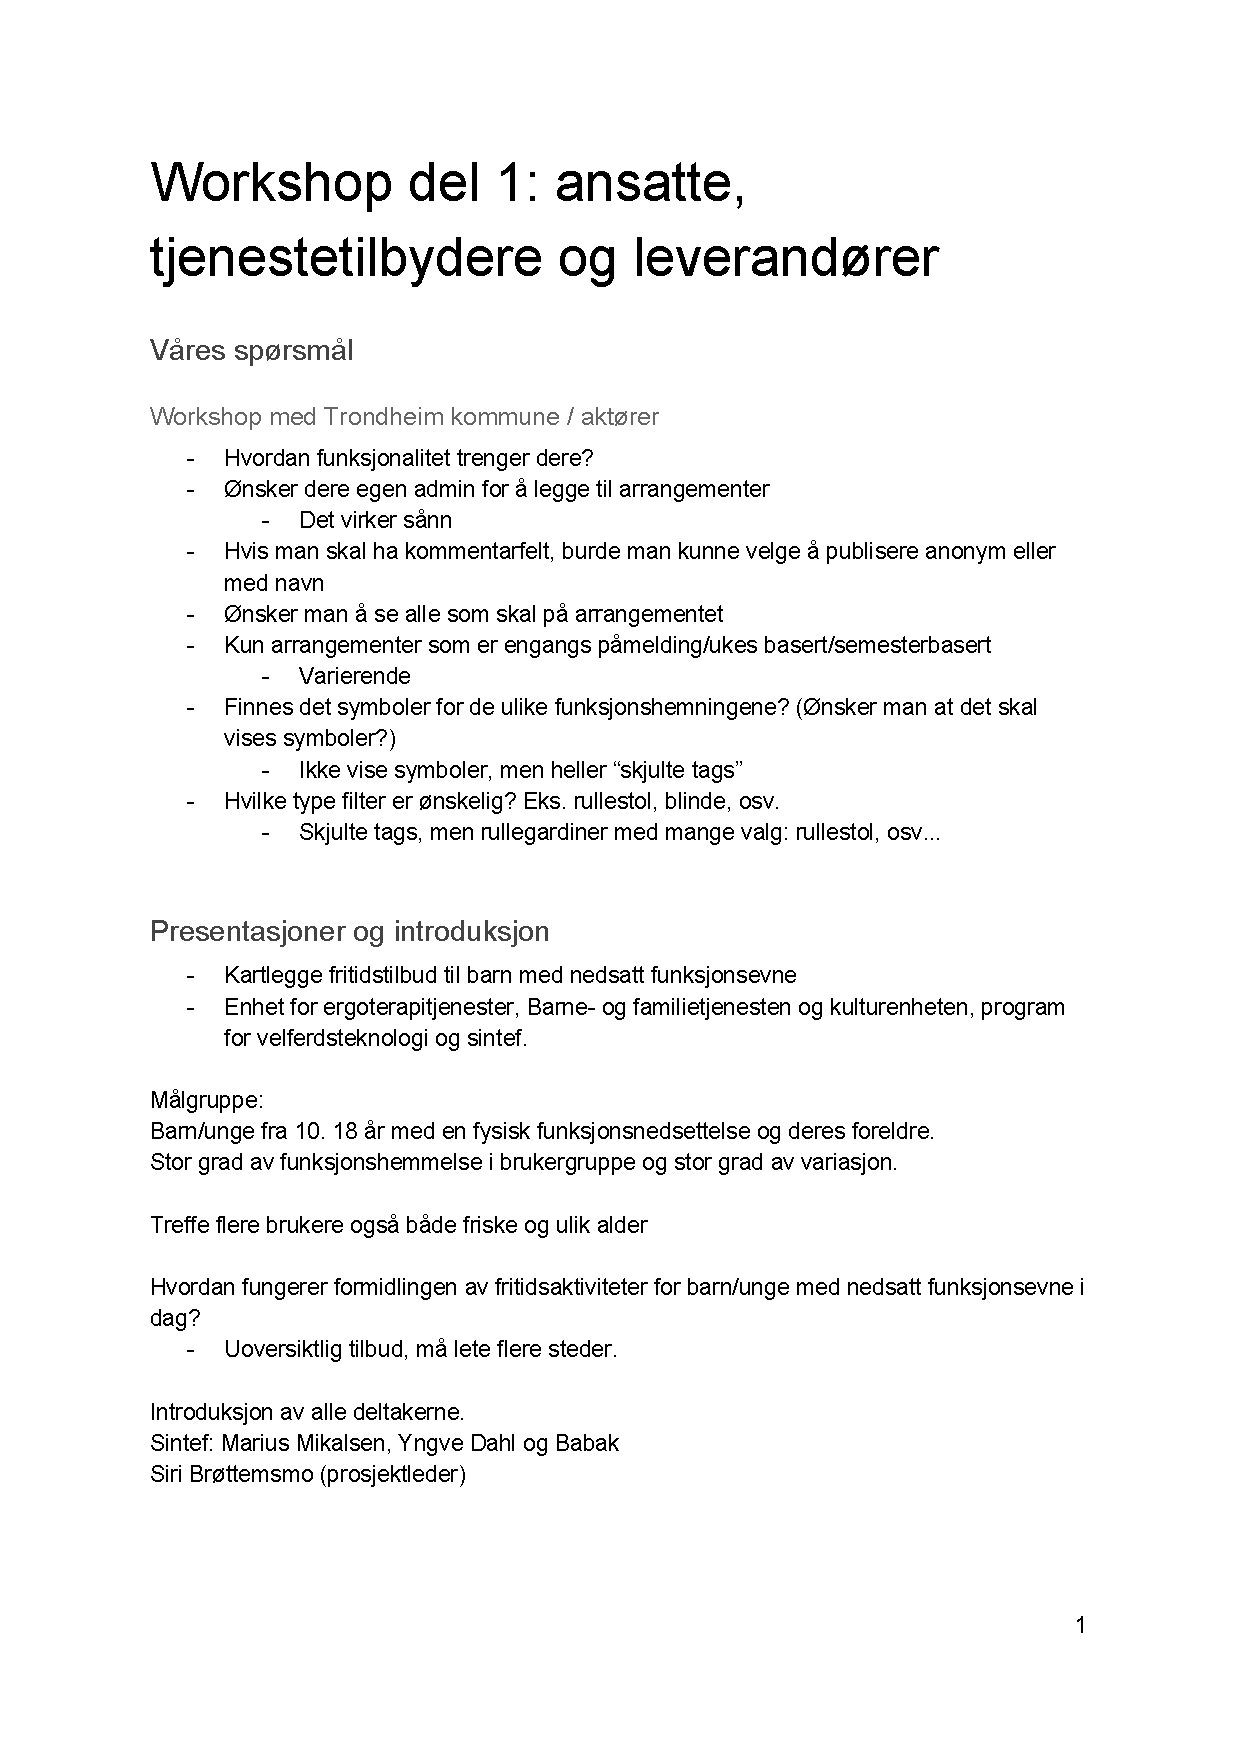
\includepdf[scale=0.9]{fig/workshop/providers/WSTilbydere_1.pdf}

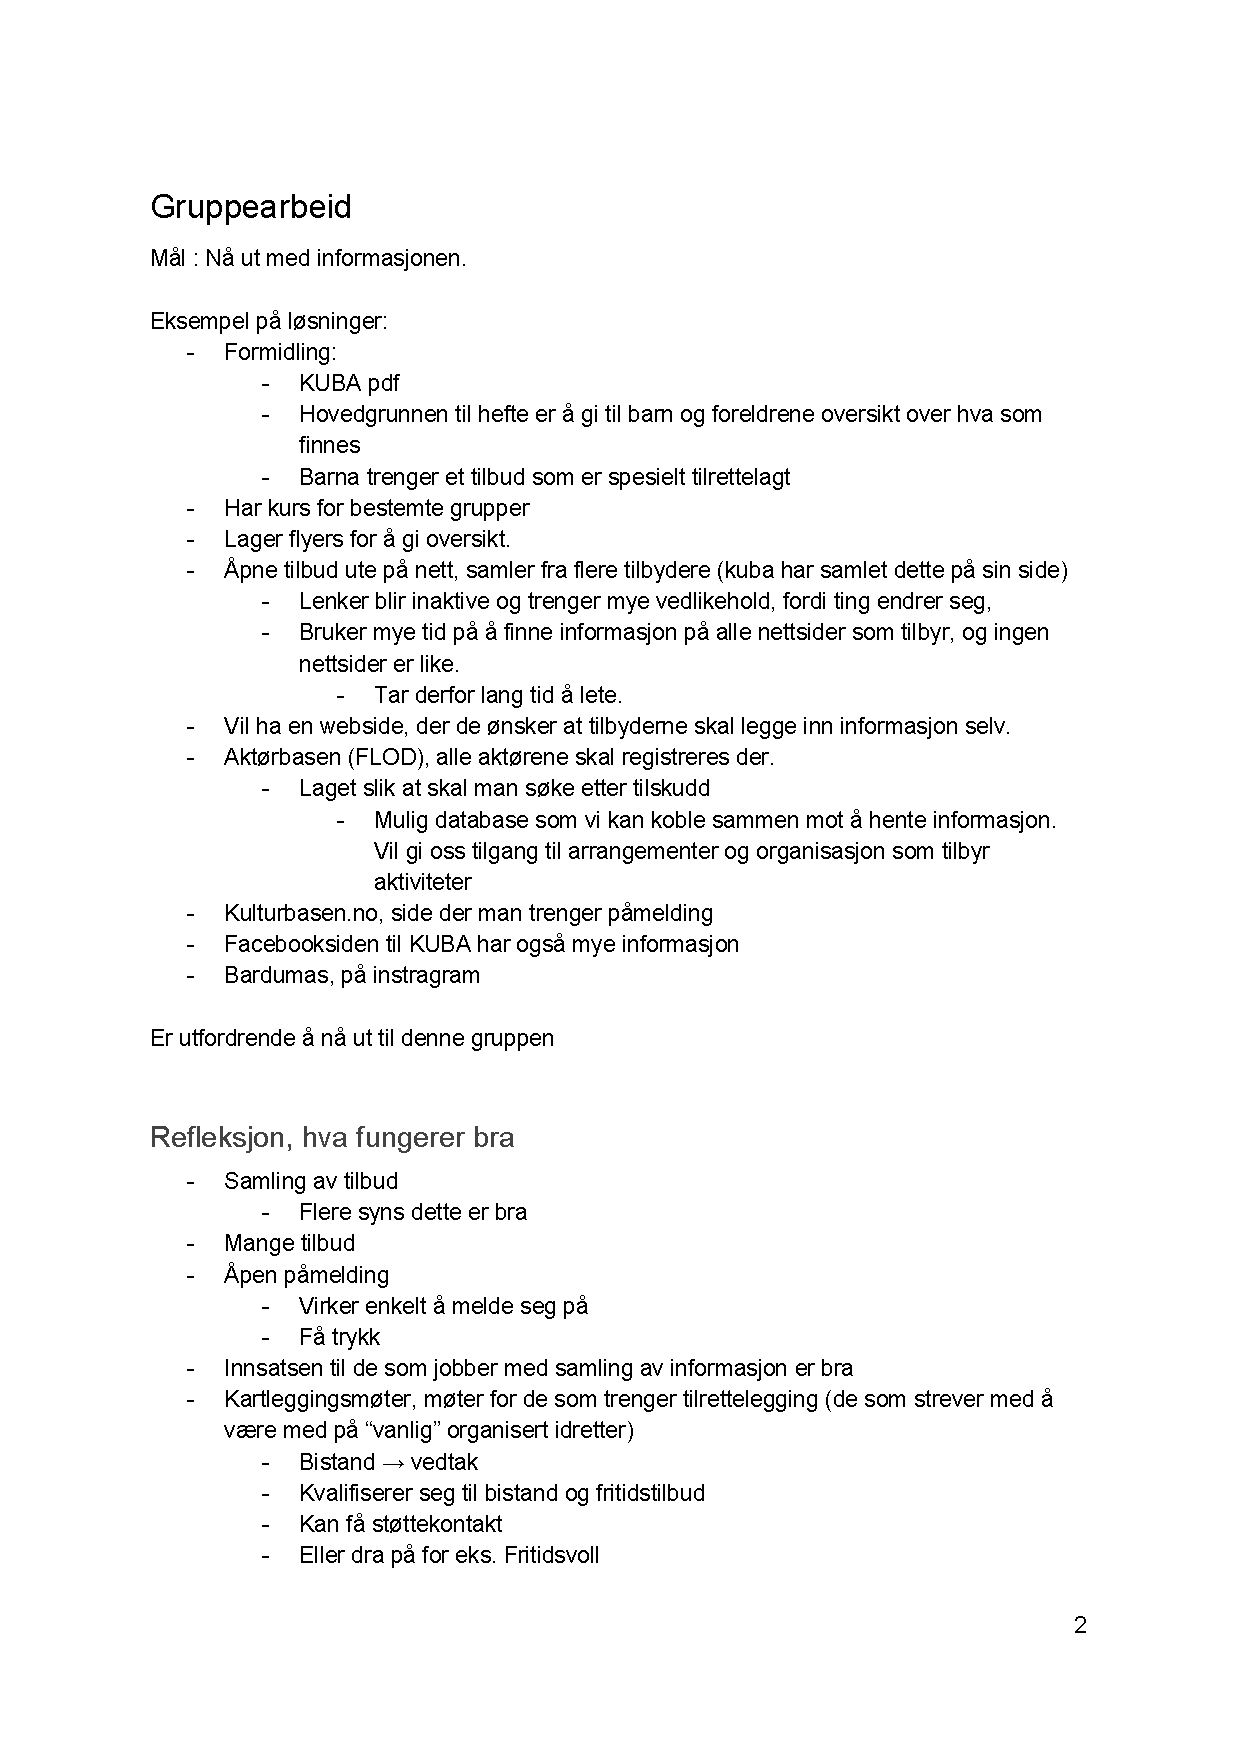
\includepdf[scale=0.9]{fig/workshop/providers/WSTilbydere_2.pdf}

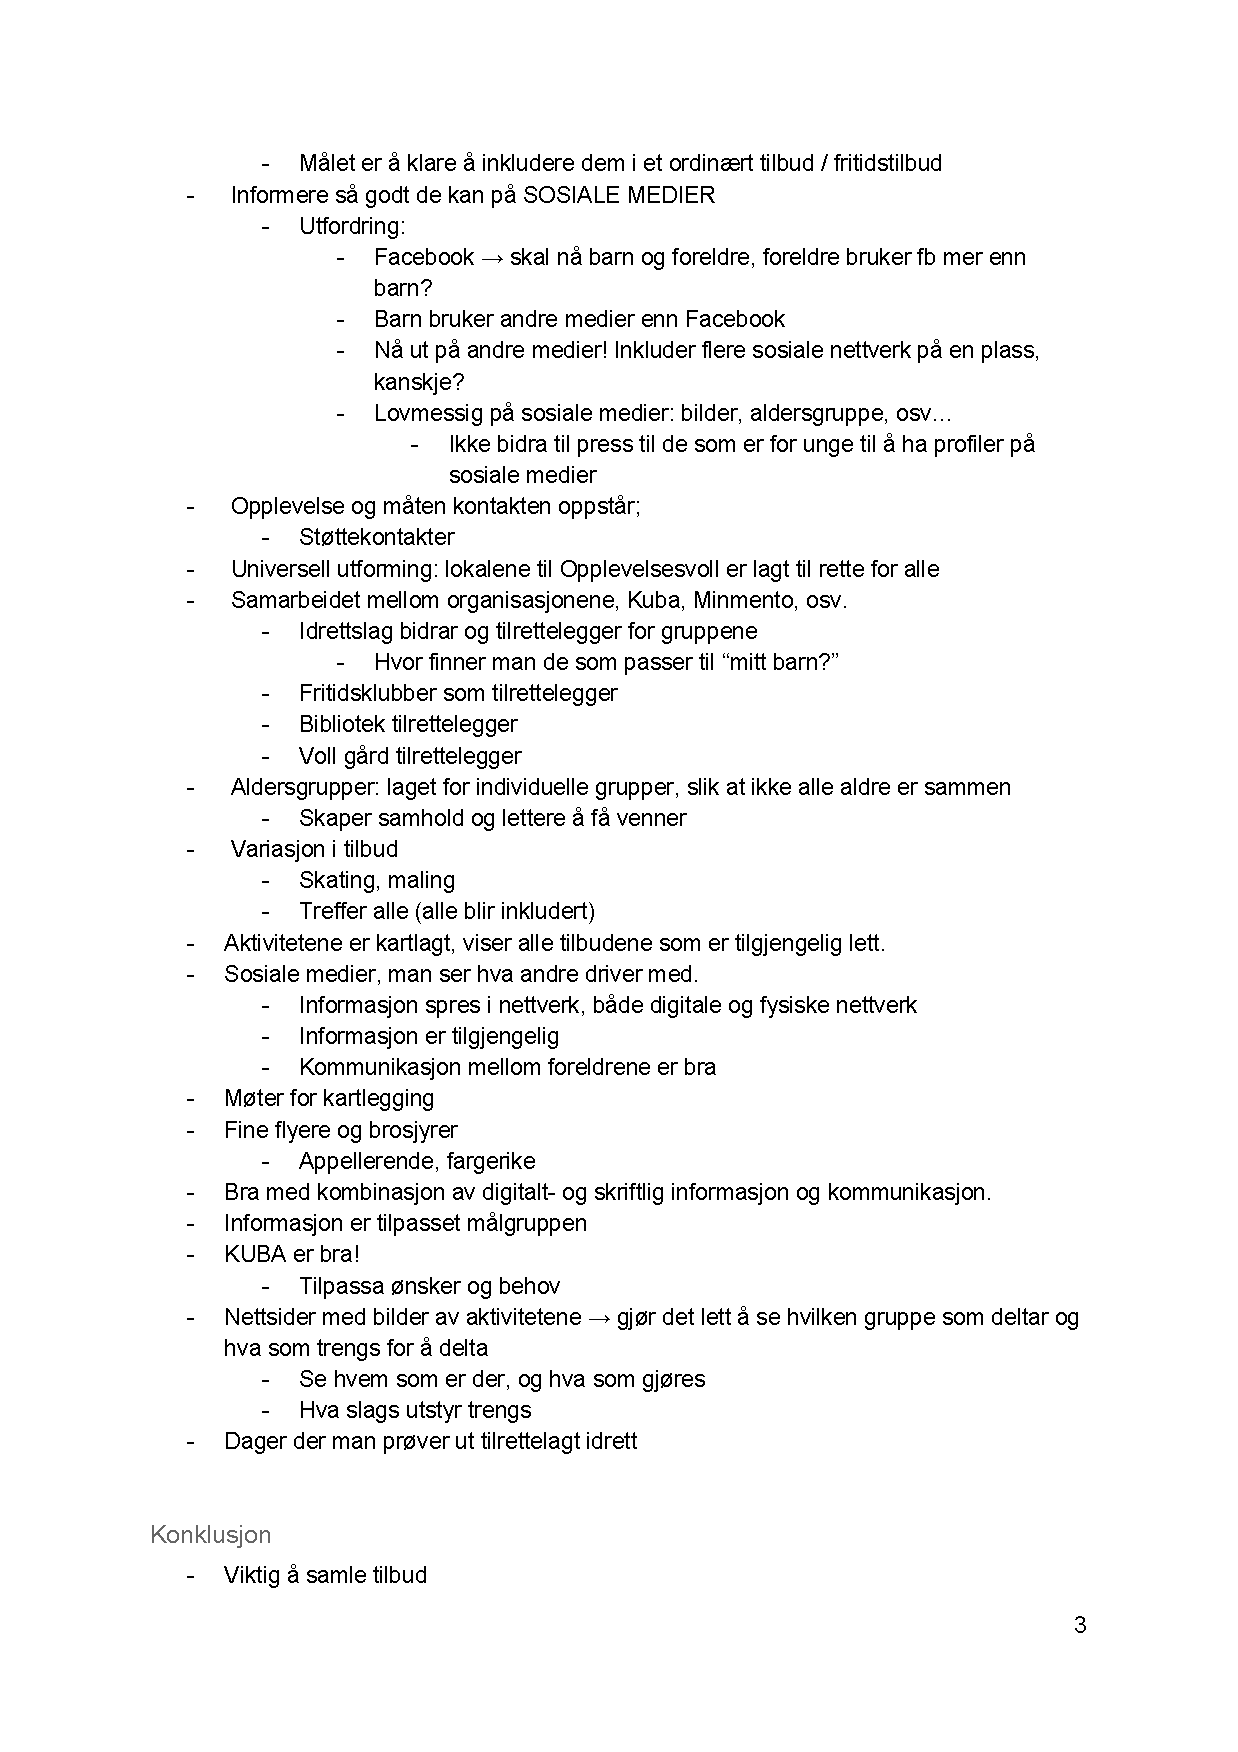
\includepdf[scale=0.9]{fig/workshop/providers/WSTilbydere_3.pdf}

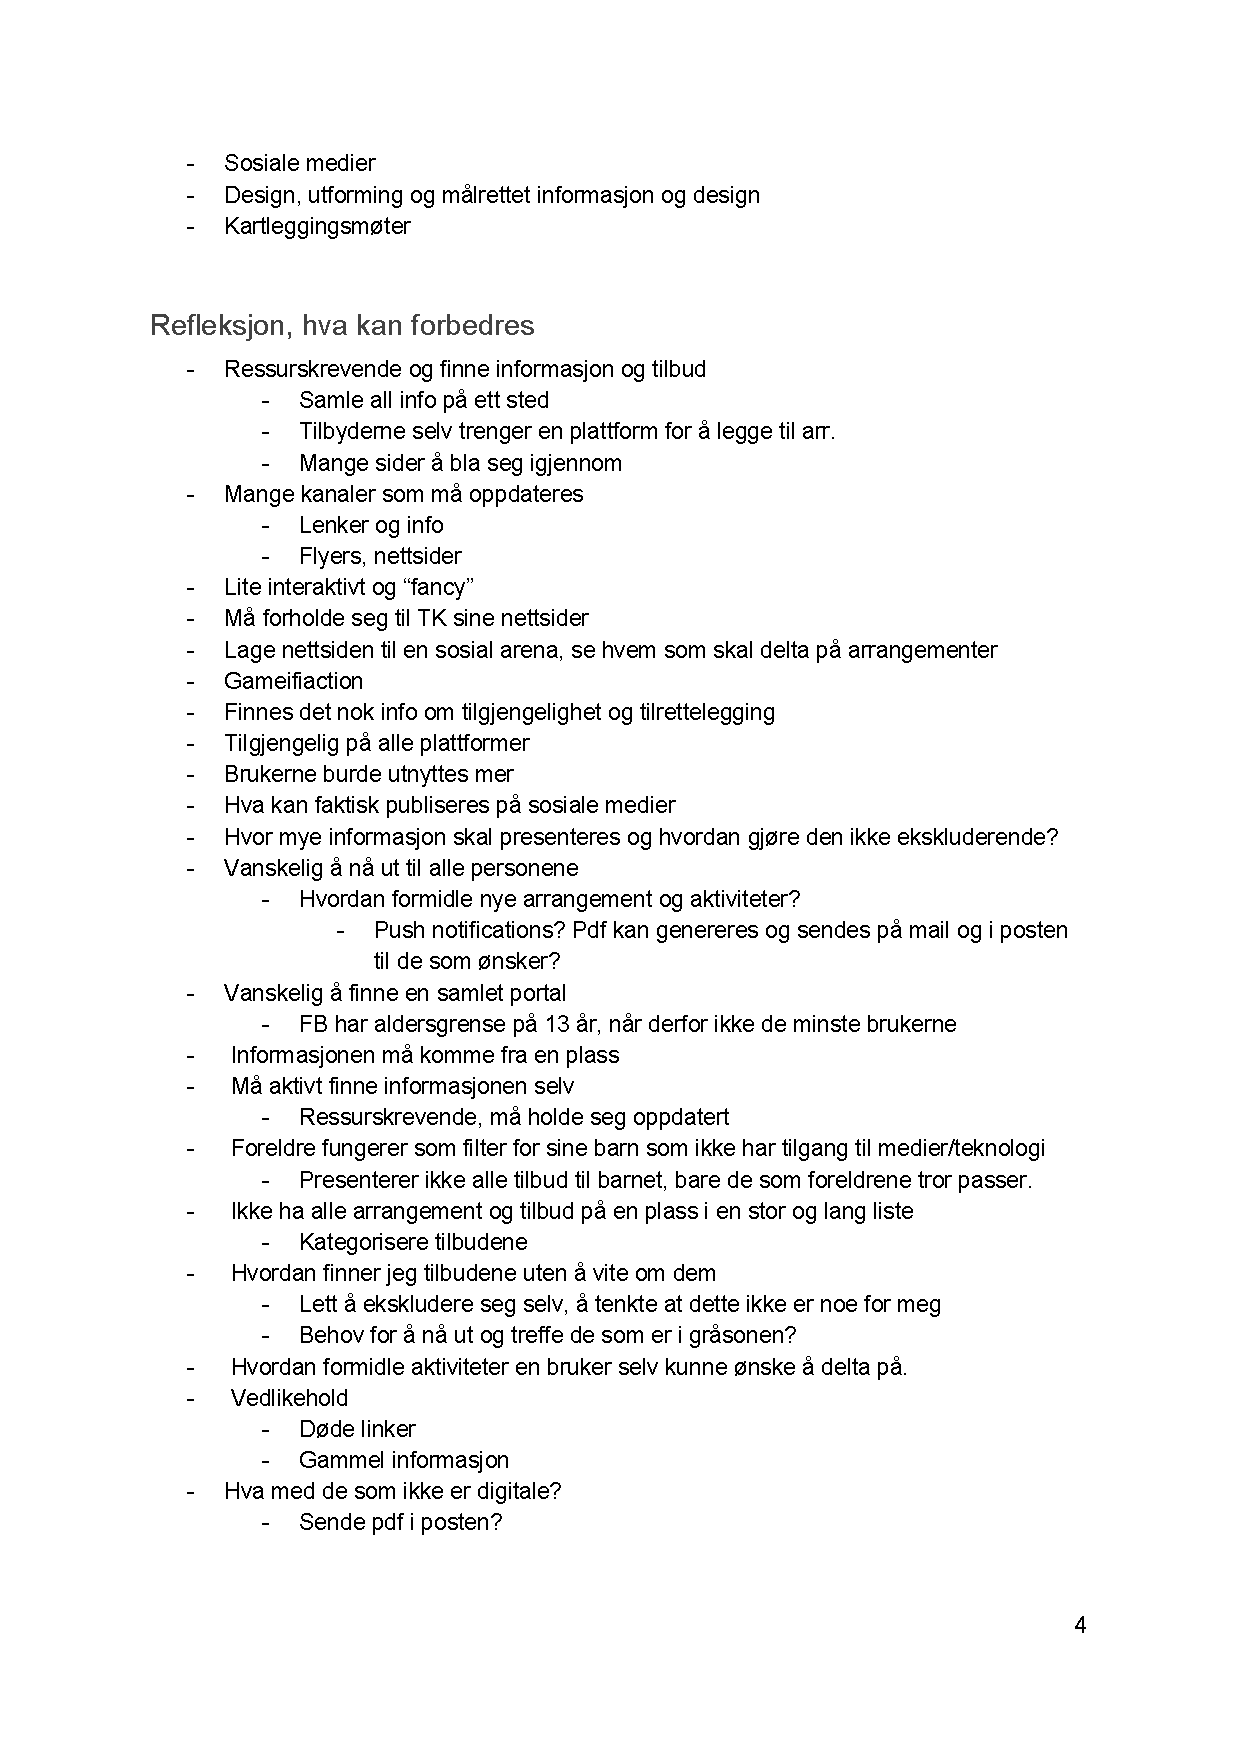
\includepdf[scale=0.9]{fig/workshop/providers/WSTilbydere_4.pdf}

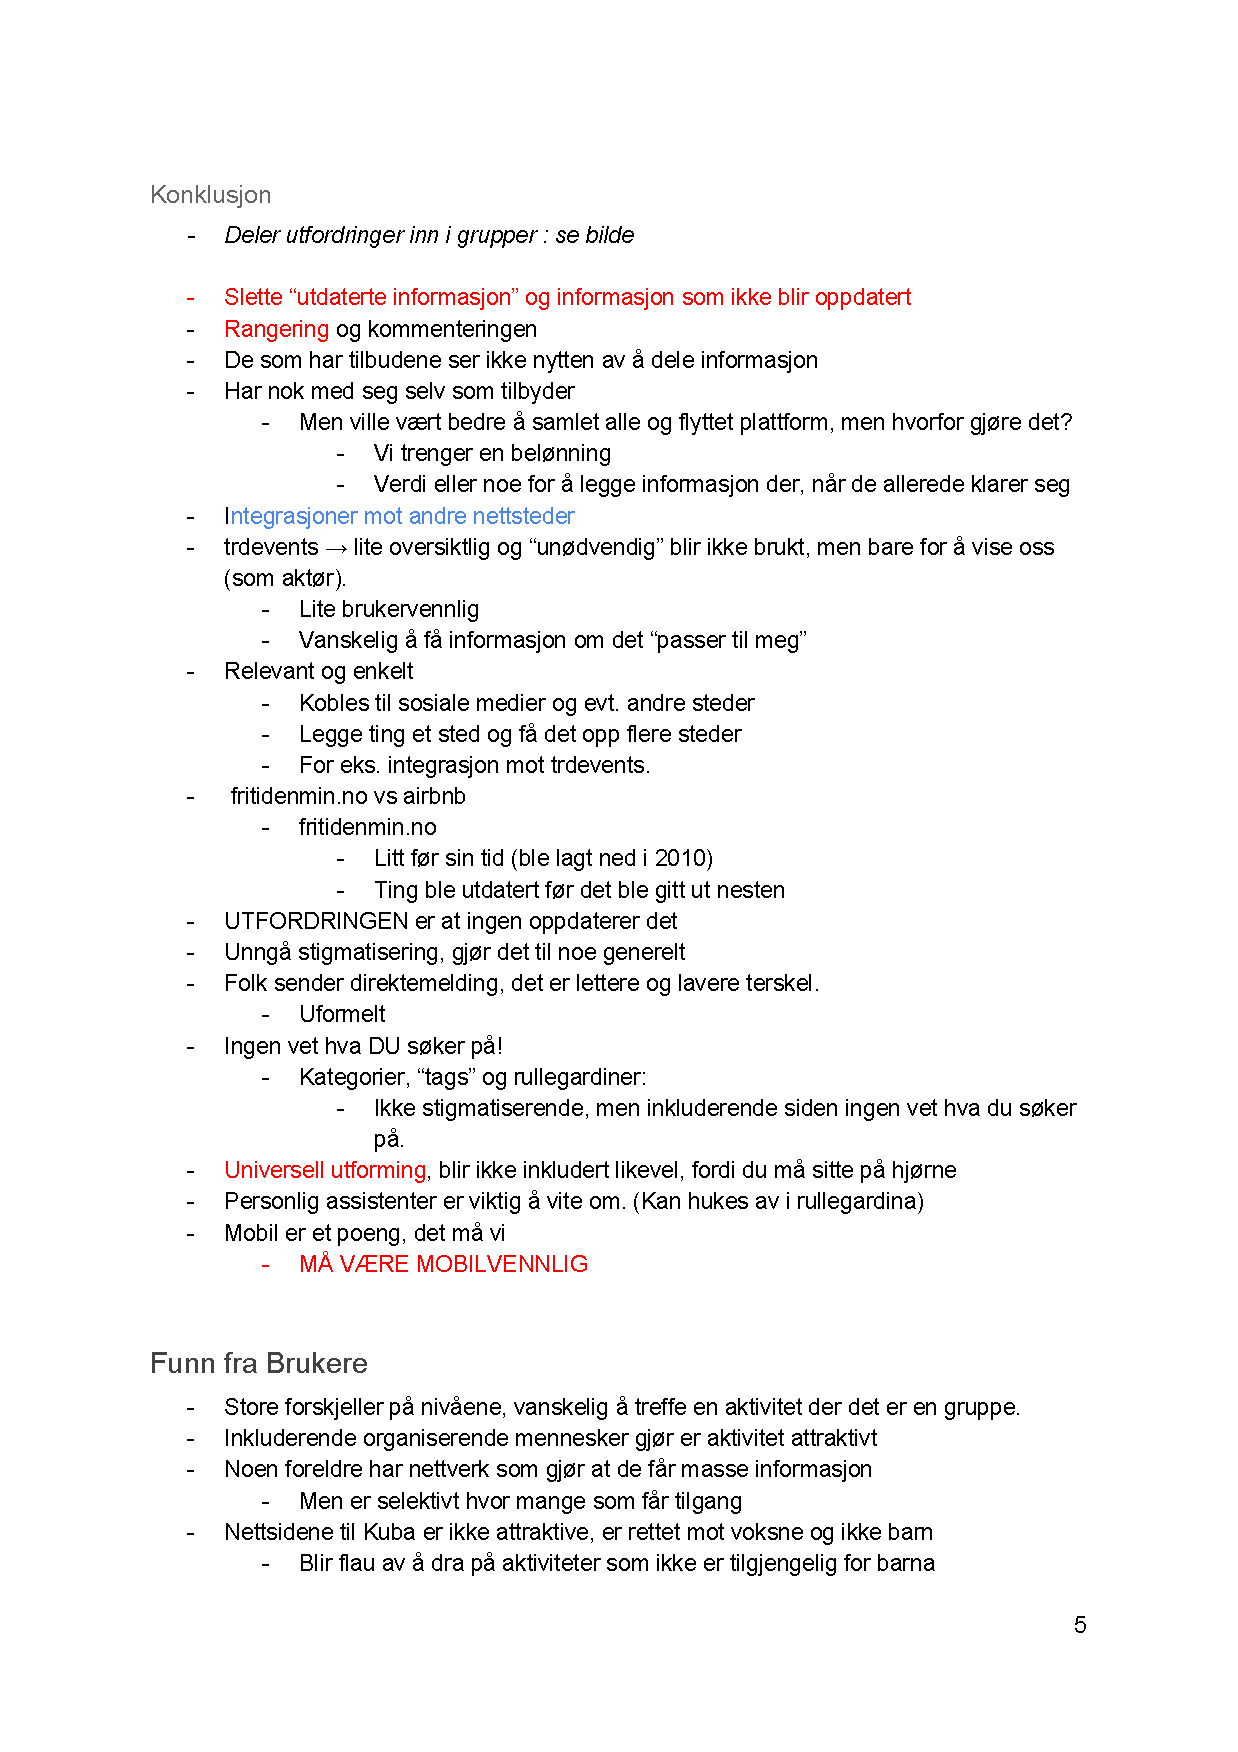
\includepdf[scale=0.9]{fig/workshop/providers/WSTilbydere_5.pdf}

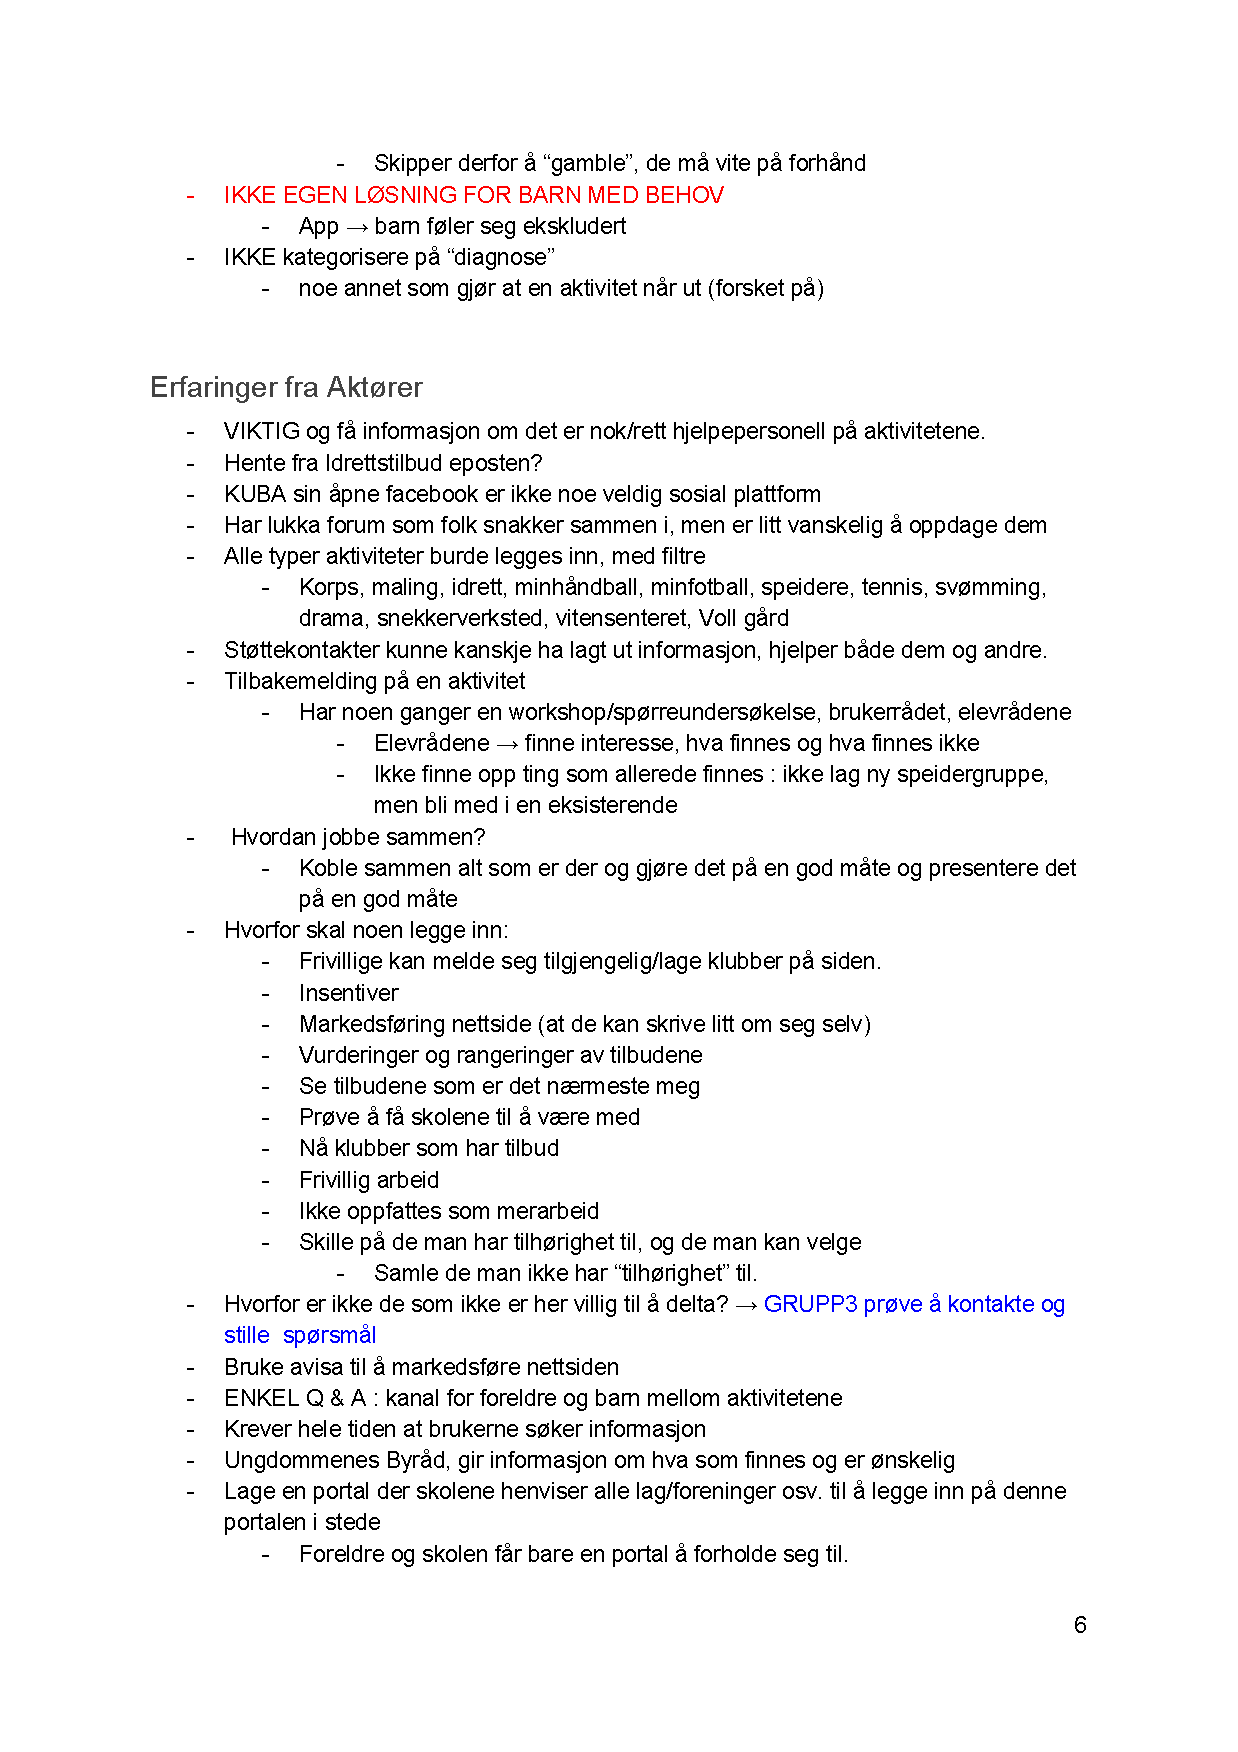
\includepdf[scale=0.9]{fig/workshop/providers/WSTilbydere_6.pdf}

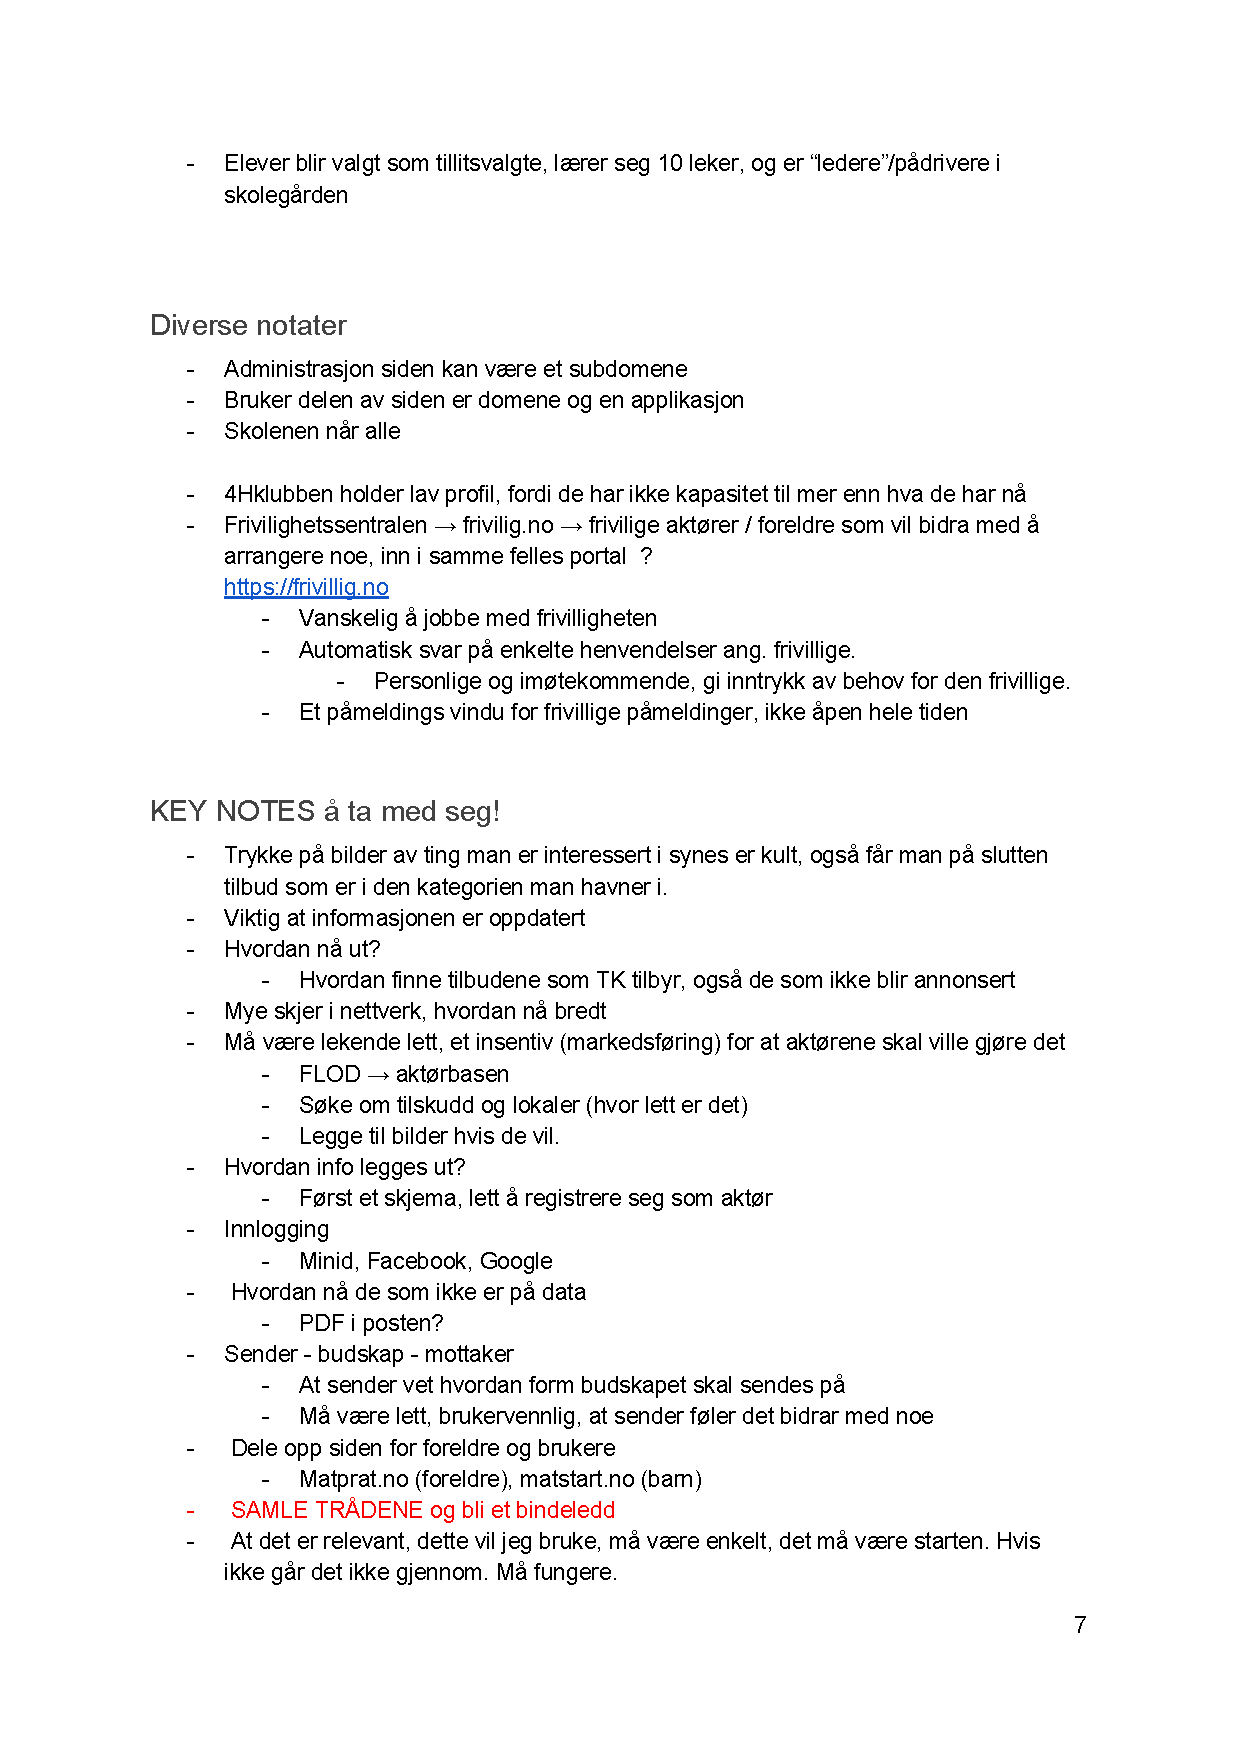
\includepdf[scale=0.9]{fig/workshop/providers/WSTilbydere_7.pdf}

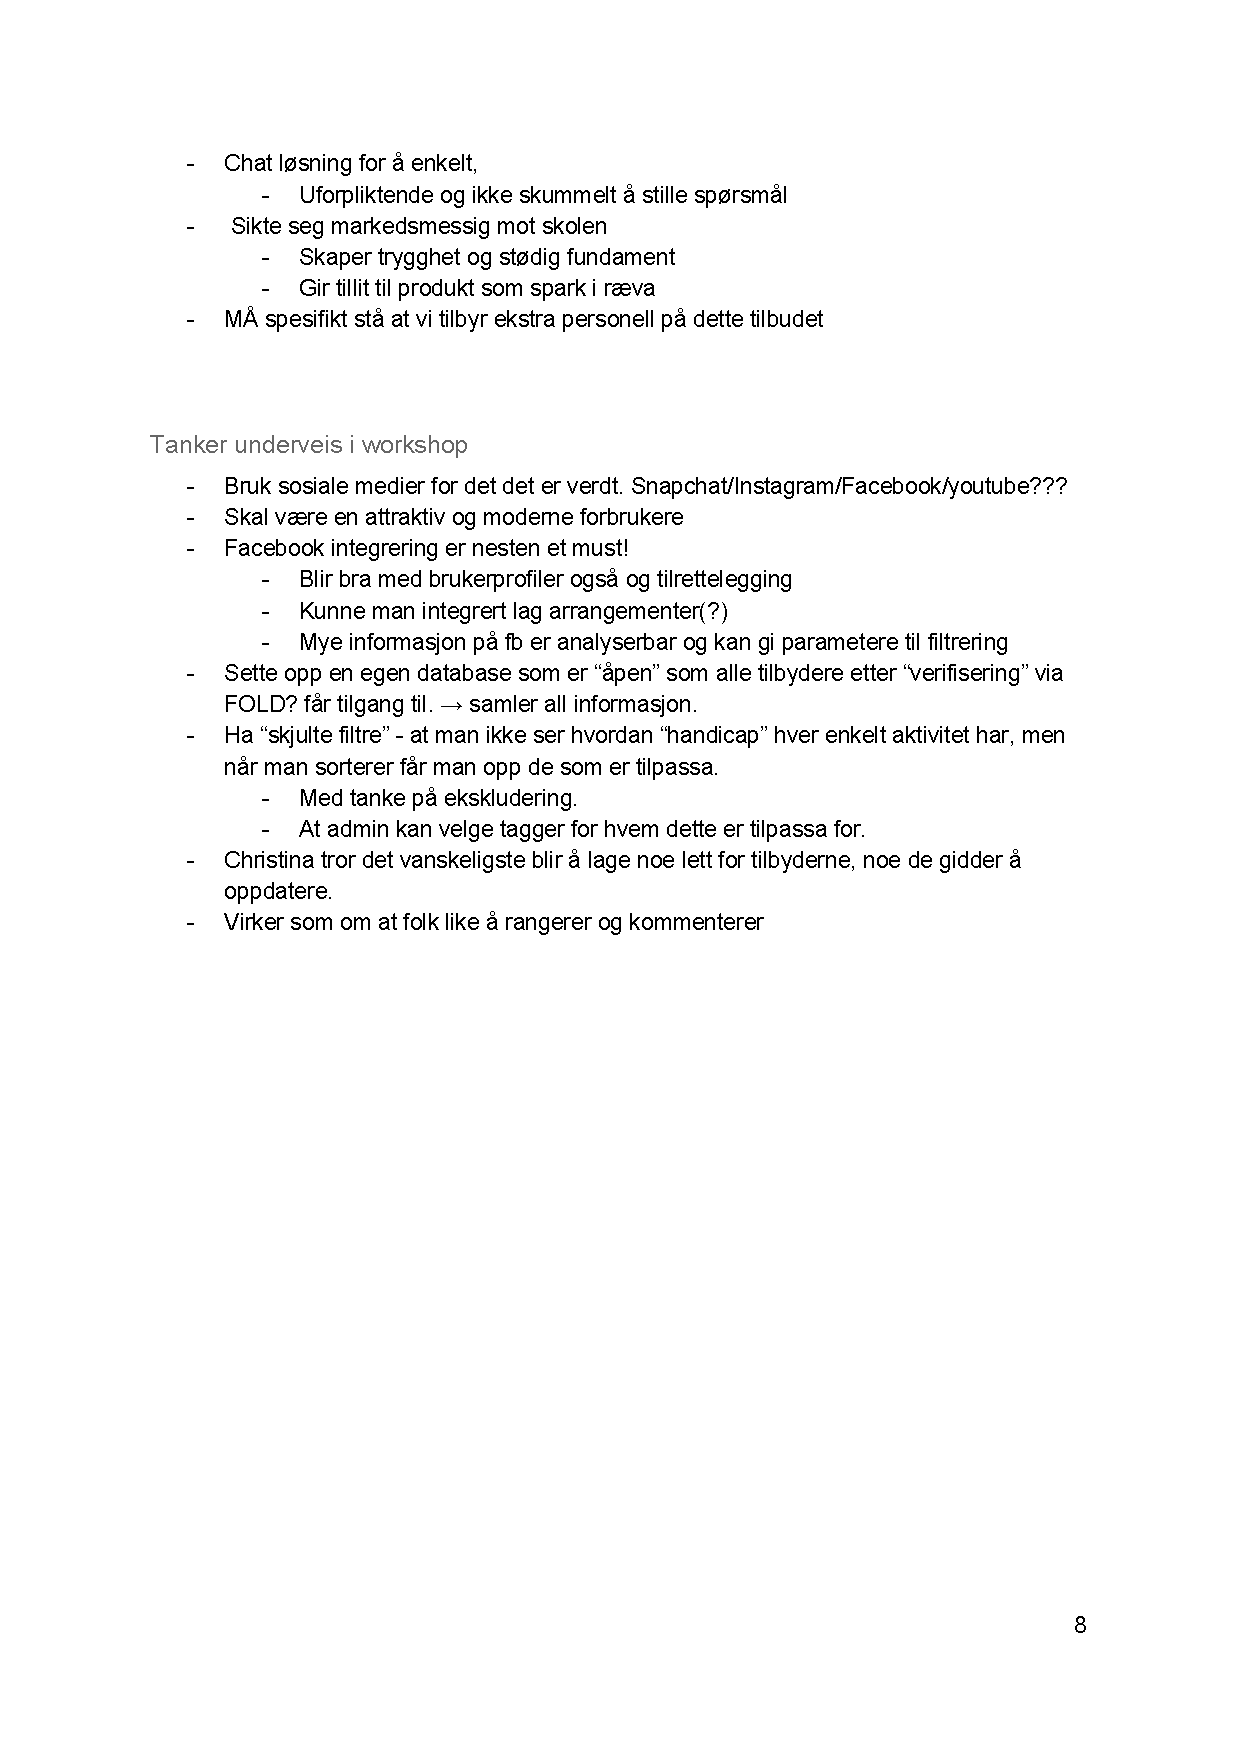
\includepdf[scale=0.9]{fig/workshop/providers/WSTilbydere_8.pdf}


\section{Workshop With Families}
\label{workshop_with_families}
The workshop were held in Norwegian and therefore the notes are in Norwegian.

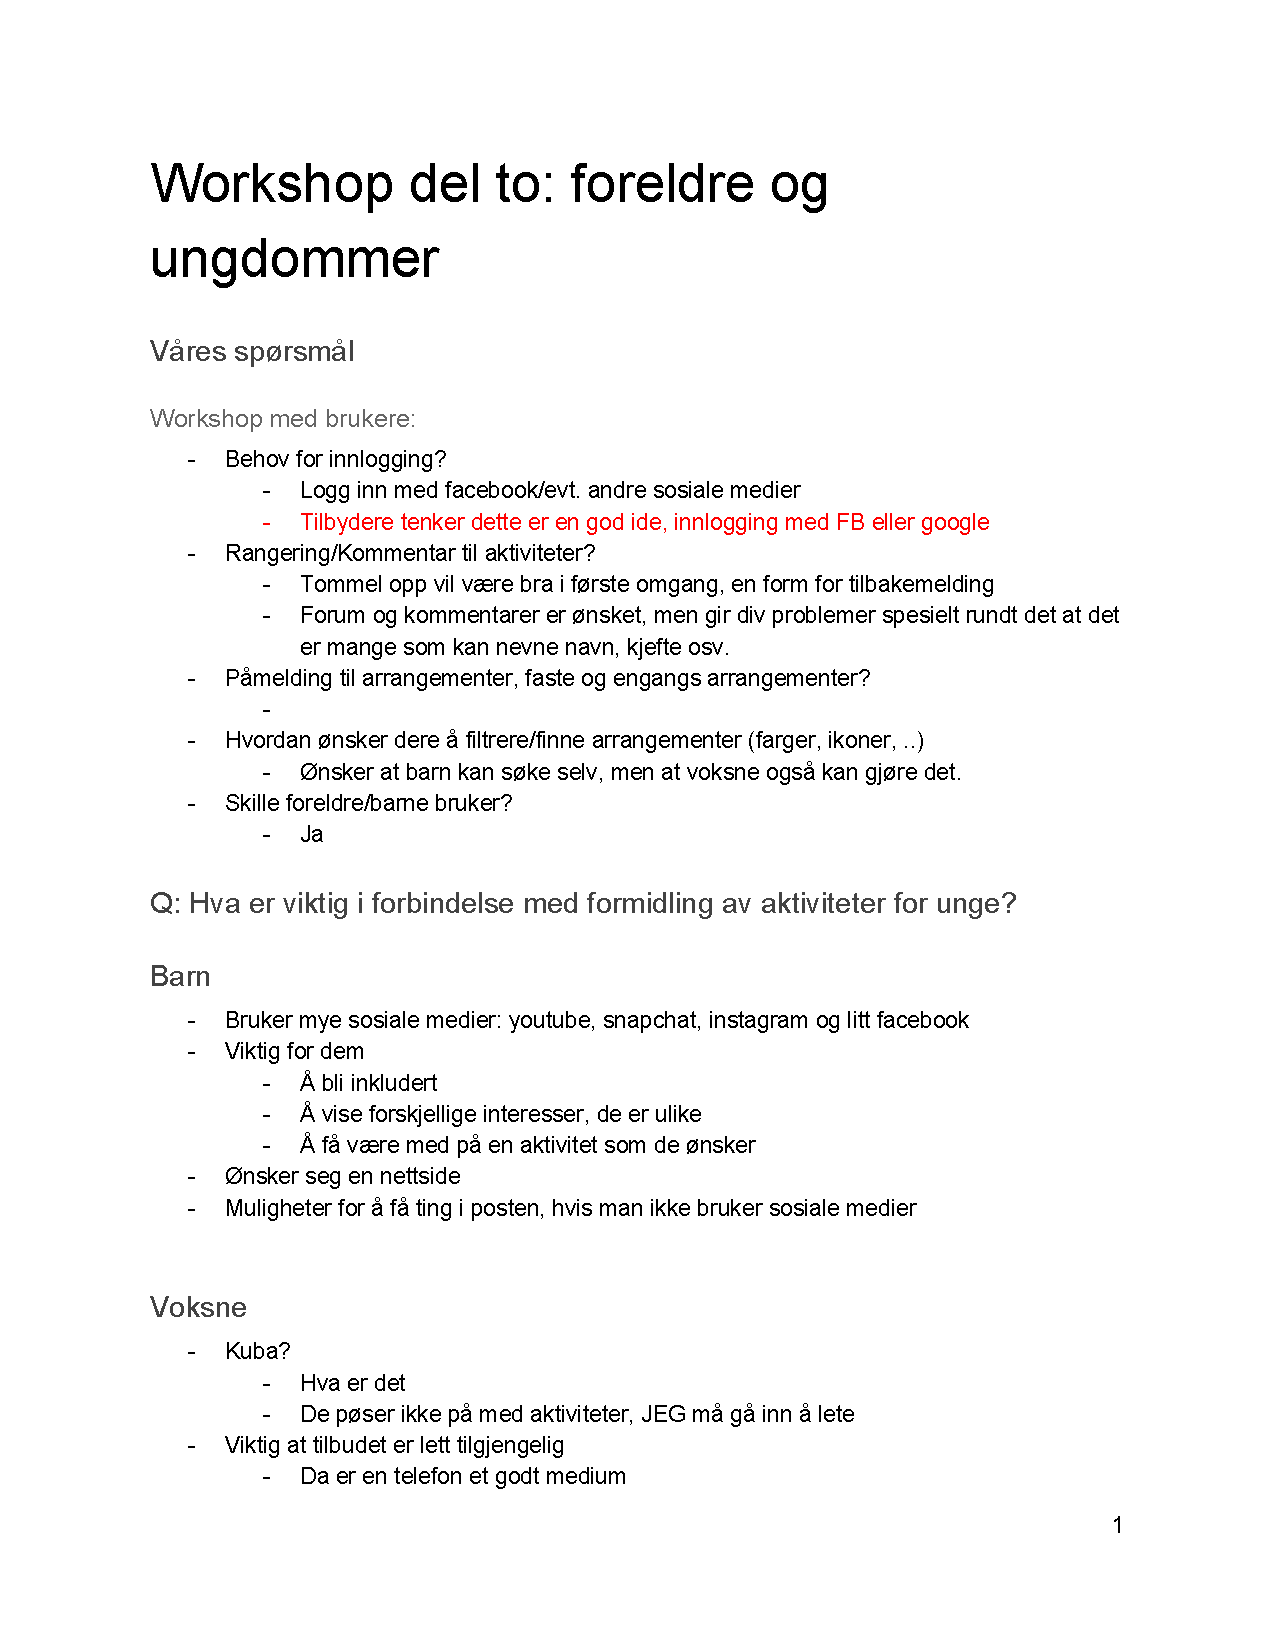
\includepdf[scale=0.9]{fig/workshop/users/WSBrukere_1.pdf}

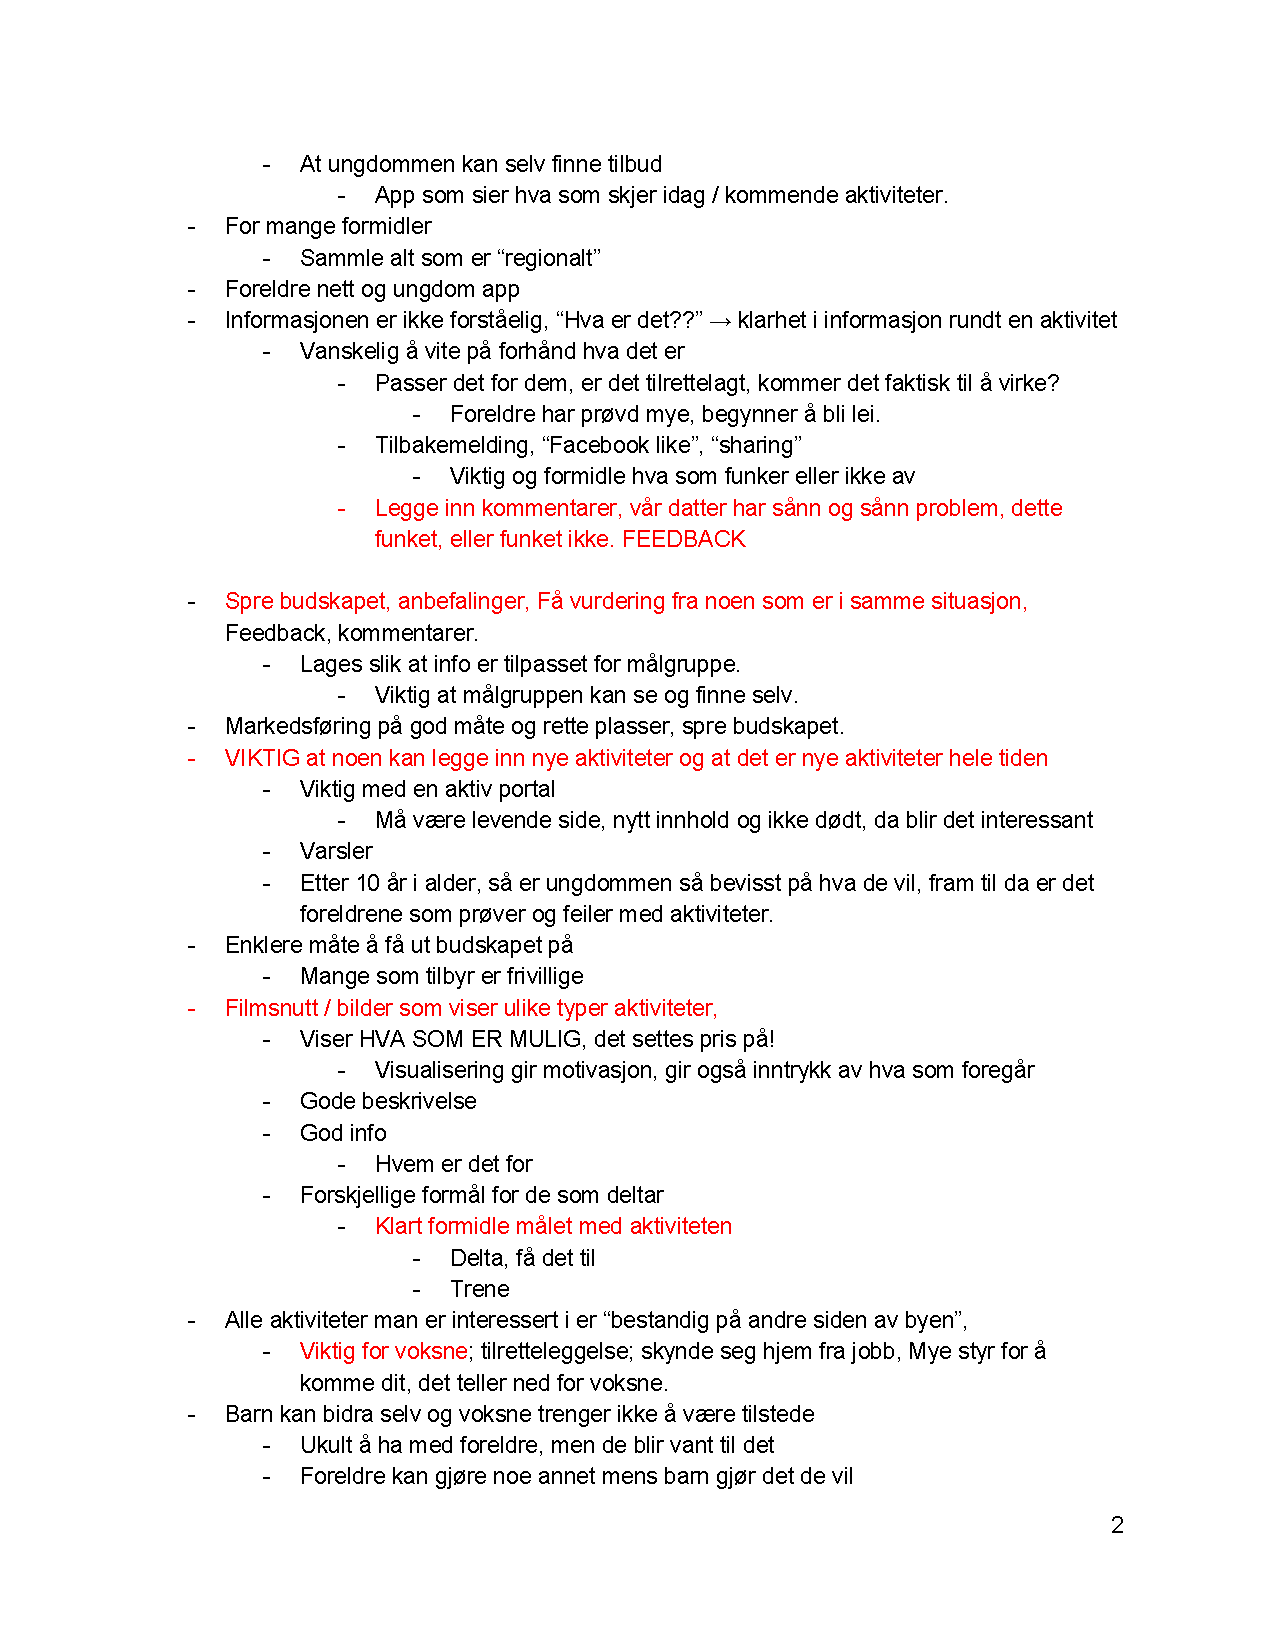
\includepdf[scale=0.9]{fig/workshop/users/WSBrukere_2.pdf}

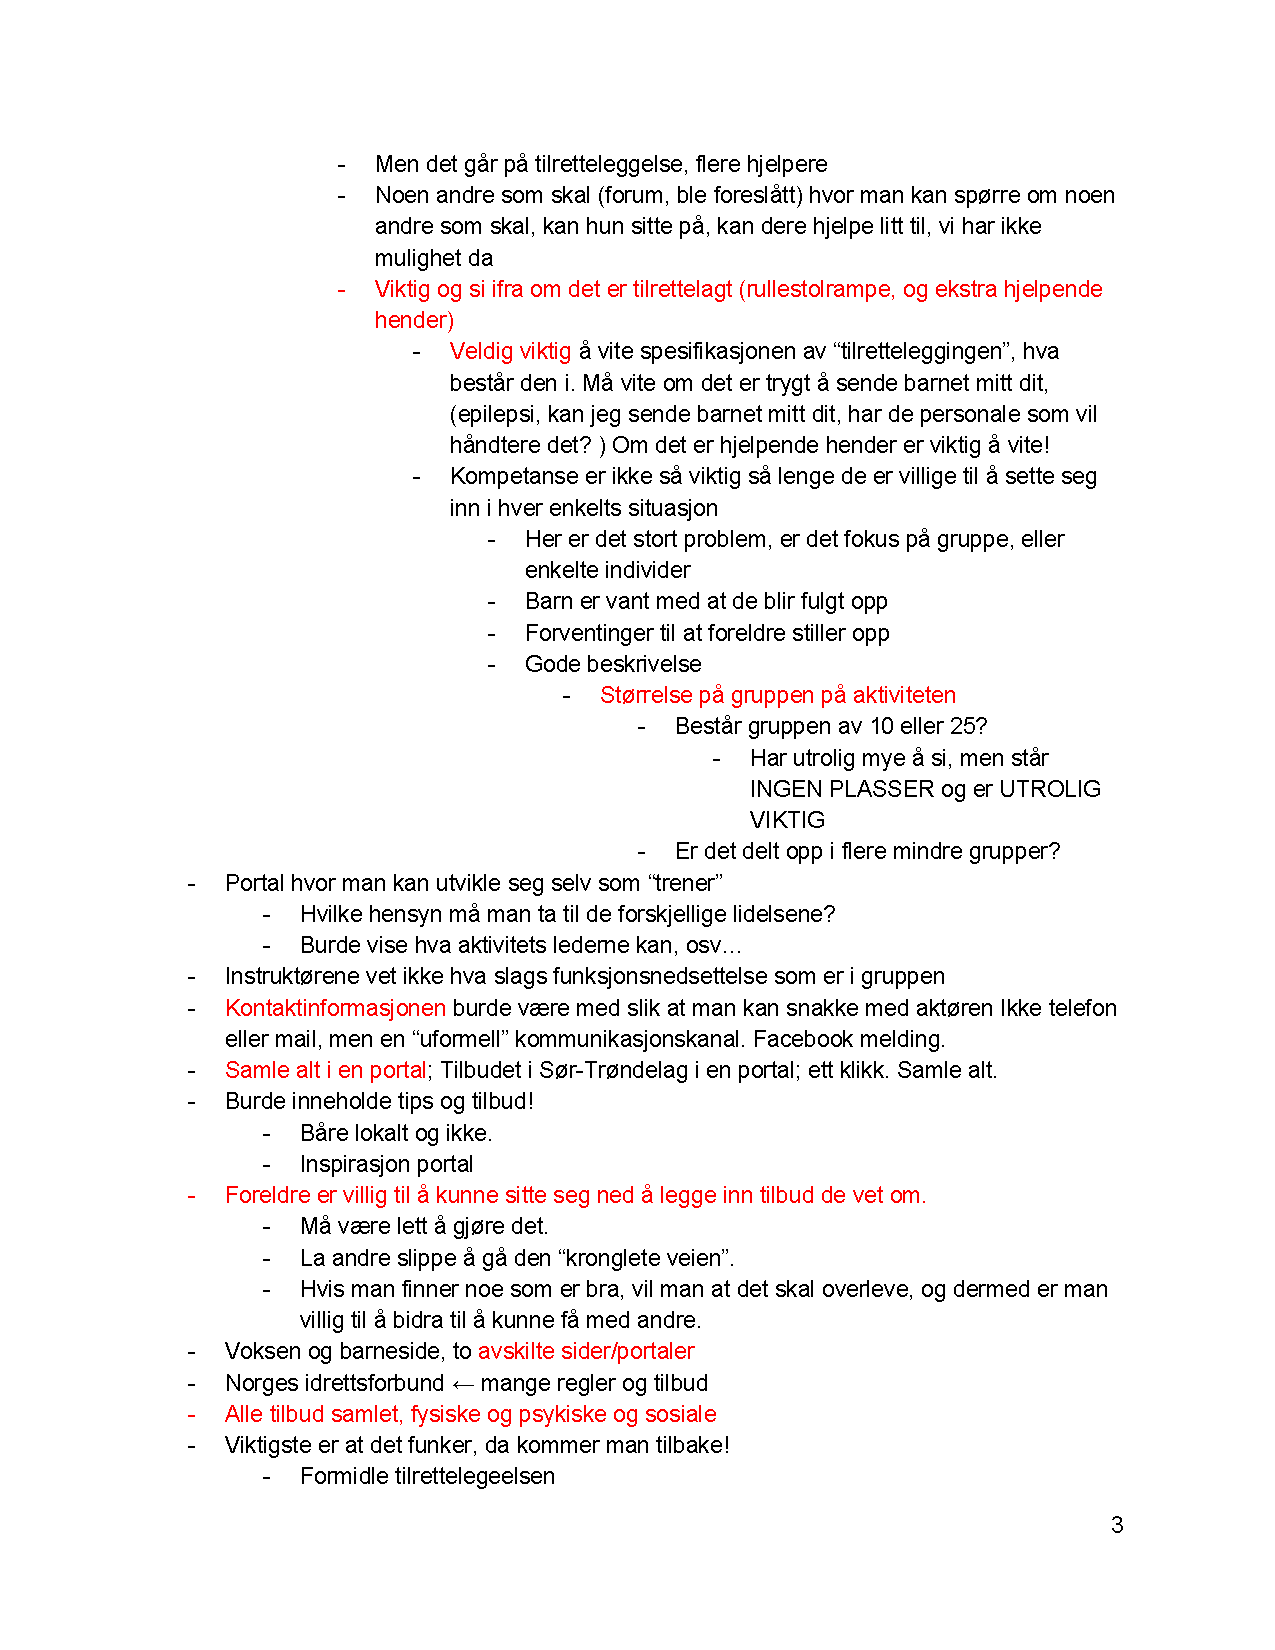
\includepdf[scale=0.9]{fig/workshop/users/WSBrukere_3.pdf}

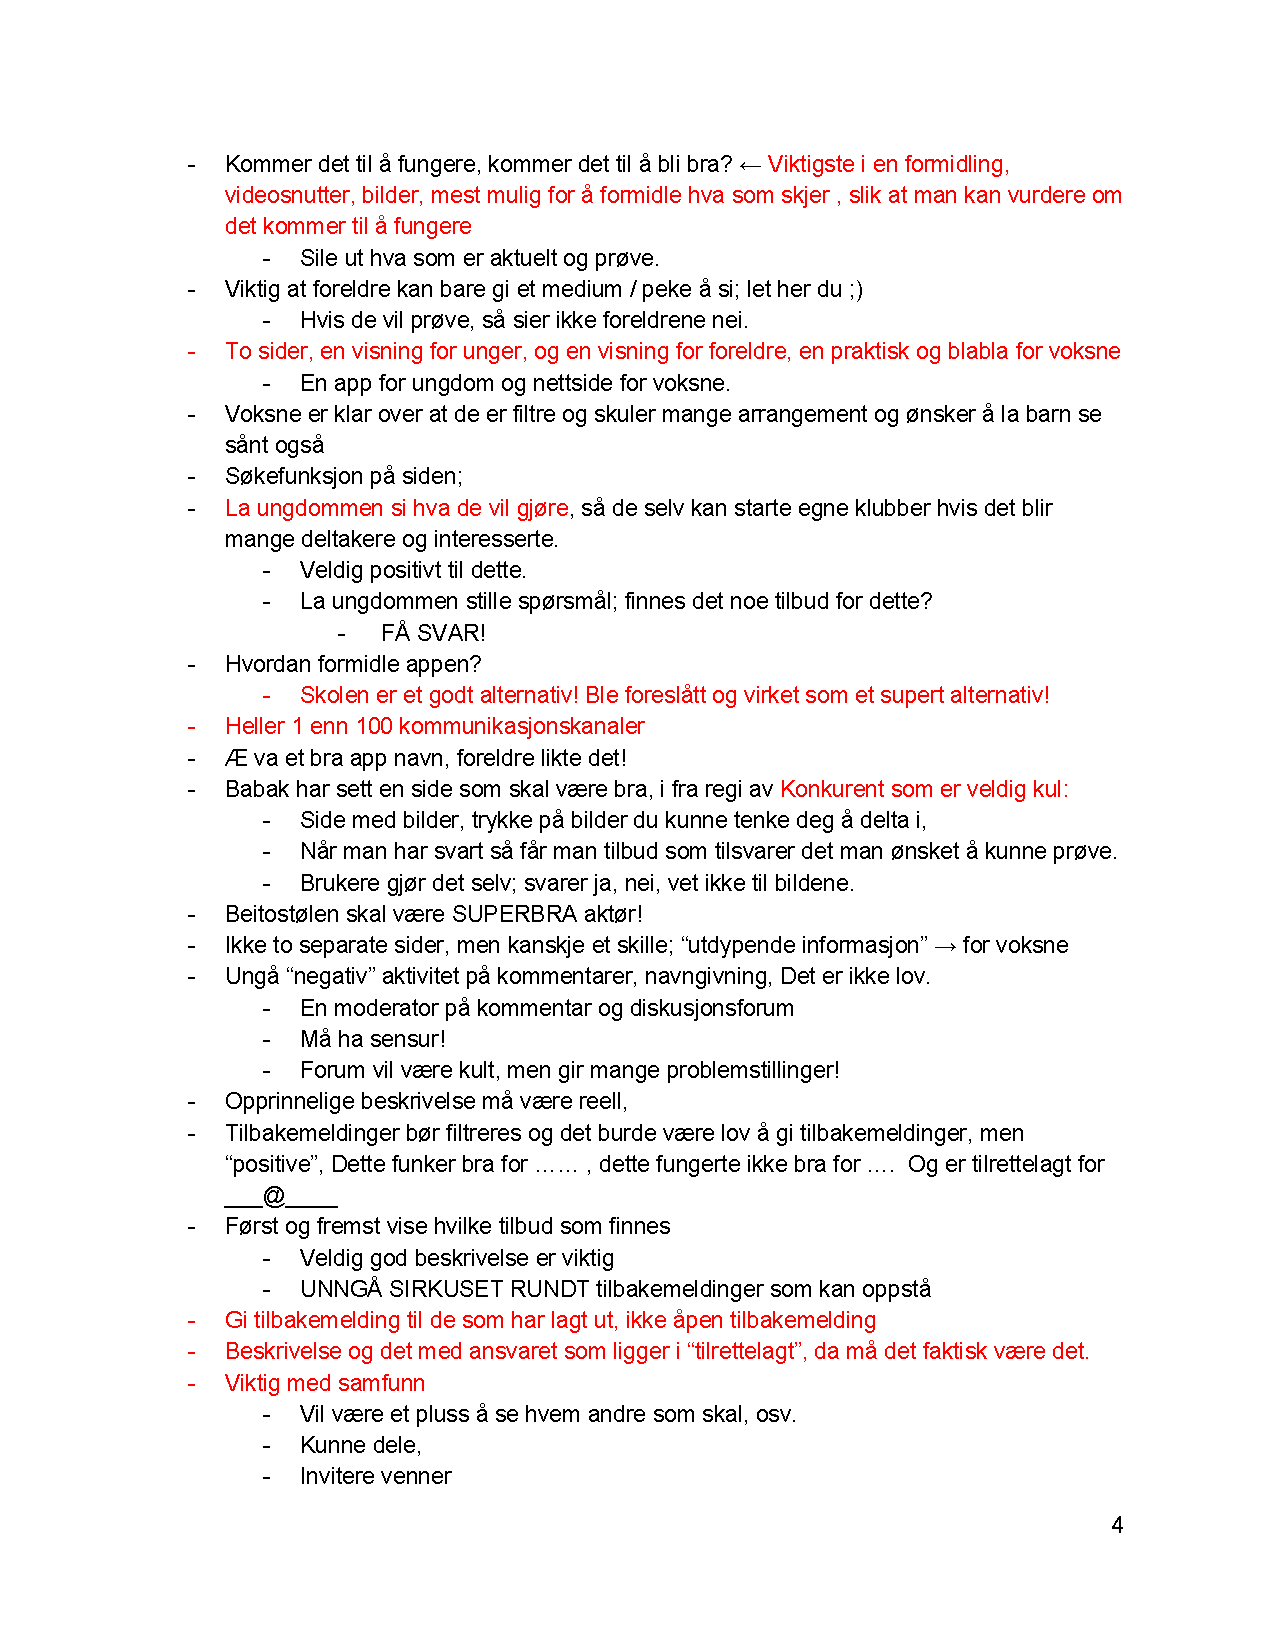
\includepdf[scale=0.9]{fig/workshop/users/WSBrukere_4.pdf}

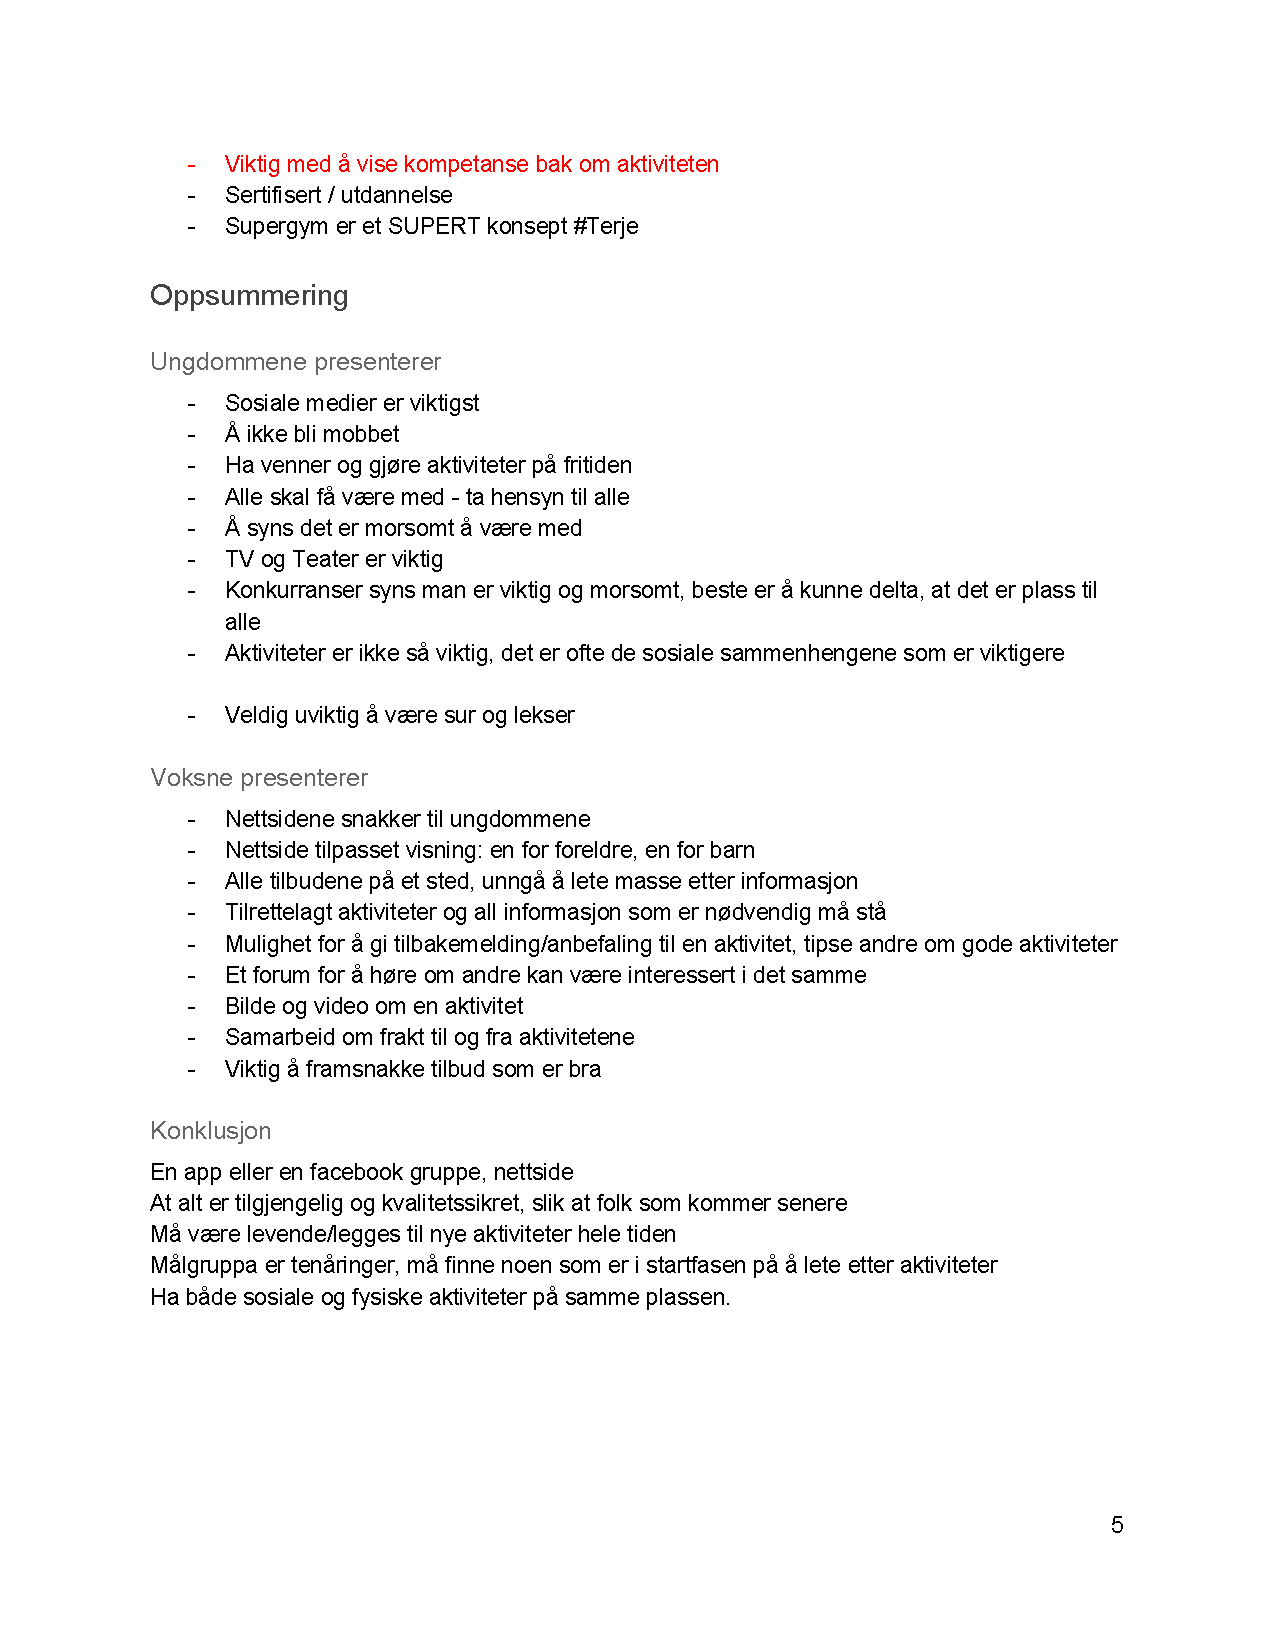
\includepdf[scale=0.9]{fig/workshop/users/WSBrukere_5.pdf}



\clearpage